\mysection[BurntOrange]{Grundbegriffe}
\DEF{Wahrscheinlichkeitstheorie}{Konstruktion mathematischer Modelle, um Aussagen über das Verhalten von Systemen zu treffen.}

\DEF{Statistik}{Identifizierung eines wahrscheinlichkeitstheoretischen Modells basierend auf beobachteten Daten.}

\DEF{Stochastik}{Die Lehre der mathematischen Beschreibung und Untersuchung zufälliger Phänomene. Wahrscheinlichkeitstheorie und Statistik zusammen, werden als Stochastik bezeichnet.}

\mysubsection{Wahrscheinlichkeitsraum}
\DEF{Zufallsexperimente}{Experimente, deren Ergebnisse nicht immer exakt vorausgesagt werden können.}

\DEF{Grundraum, Ereignisraum (sample Space) $\Omega$}{Menge aller möglichen Ergebnisse des betrachteten Zufallsexperiments. Es gilt $\Omega\neq\emptyset$.}

\DEF{Elementarereigniss, Ausgänge des Experiments (outcomes)}{Elemente $\omega\in\Omega$.}

\DEF{Potenzmenge (power set)}{Potenzmenge $\mathcal{P}(\Omega
) = 2^\Omega = \{X|X\subseteq\Omega\}$ ist die Menge aller Teilmengen von $\Omega$. Es gilt $|\mathcal{P}(\Omega)|= 2^{|\Omega|}$.}

\DEF{Prinzipielles/mögliches Ereignis (event)}{Eine Teilmenge $\mathcal{A}\subseteq\Omega$. Wir sagen, das Ereignis $\mathcal{A}$ tritt ein, falls das realisierte Elementarereignis $\omega$ in $\mathcal{A}$ liegt ($\omega\in\mathcal{A})$. $A=\emptyset$ tritt nie ein. $A=\Omega$ tritt immer ein.}

\DEF{$\sigma$-Algebra}{Die Klasse aller beobachtbaren Ereignisse $\mathcal{F}\subseteq\mathcal{P}(\Omega)$. Axiome:
\begin{enumerate}
    \item $\Omega\in\mathcal{F}$.
    \item $A\in\mathcal{F} \Leftrightarrow A^C\in\mathcal{F}$.
    \item Sei $(A_n)_{n\in\N}$ eine beliebige Folge. Dann $A_n\in\mathcal{F}$ $\forall$ $n\in\N \Leftrightarrow \bigcup_{n\in\N}A_n\in\mathcal{F}$.
\end{enumerate}

Daraus folgt
\begin{enumerate}
    \item Sei $(A_n)_{n\in\N}$ eine beliebige Folge. Dann $A_n\in\mathcal{F}$ $\forall$ $n\in\N \Rightarrow \bigcap_{n\in\N}A_n\in\mathcal{F}$
\end{enumerate}}

\DEF{Borelsche $\sigma$-Algebra auf $\R$}{Beinhaltet alle Mengen, welche in dieser Vorlesung interessieren. Folgenden Mengen sind Elemente von $\mathcal{B}(\R)$:
\begin{itemize}
    \item alle offenen, abgeschlossenen und kompakten Mengen $\in\R$.
    \item alle Intervalle der Form $(a,b)$, $[a,b]$, $(a,b]$, $[a,b)$, $(-\infty,b)$, $-\infty,b]$, $(a,\infty)$, $[a,\infty)$ für $a,b\in\R$.
\end{itemize}}

\DEF{Wahrscheinlichkeitsmass (probability measure)}{$\P$ auf $(\Omega, \mathcal{F})$ ist eine Abbildung $\P:\mathcal{F}\rightarrow[0,1]$ mit $A\mapsto\P[A]$, wobei folgende Axiome erfüllt sind.

Axiome:
\begin{enumerate}[nolistsep]
    \item $\P[\Omega]=1$ (normiertheit).
    \item $\P[\bigcup_{n\in\N}A_n]=\sum_{n=1}^\infty\P[A_n]$ für paarweise disjunkte Mengen $A_n$, d.h. $A_n\cap A_m = \emptyset$ $\forall$ $n\neq m$ ($\sigma$-Additivität).
\end{enumerate}

Rechenregeln: \begin{enumerate}
    \item $\P[A^C]=1-\P[A]$.
    \item $A\subseteq B \Rightarrow \P[A]\leq\P[B]$ (monotonie).
    \item $\P[A] + \P[B] = \P[A\cup B] + \P[A\cap B]$ (Additionsregel).
\end{enumerate}}

$\P$ ordnet jedem Ereignis $A$ der $\sigma$-Algebra $\mathcal{F}$ eine Wahrscheinlichkeit (Zahl zwischen $0$ und $1$) zu.

\DEF{Siebformel, Prinzip der Inklusion/Exklusion}{Seien $A_1,...,A_n\in\mathcal{F}$ beliebig ($n\geq 2$). Dann $\P[\bigcup_{i=1}^nA_i]=\sum_{k=1}^n(-1)^{k+1}\sum_{1\leq i_1<...<i_k\leq n}\P[\bigcap_{j=1}^kA_{i_j}] = \sum_{k=1}^n(-1)^{k+1}\sum_{J\subseteq \{1,...,n\}, |J|=k}\P[\bigcap_{j\in J}A_{j}]$. Der Fall $n=2$ entspricht genau der Additionsregel. Für $n=3$ gilt $\P[A_1 \cup A_2 \cup A_3]=\P[A_1]+\P[A_2]+\P[A_3]-\P[A_1\cap A_2]-\P[A_1\cap A_3]-\P[A_2\cap A_3]+\P[A_1\cap A_2 \cap A_3]$.}

\DEF{Boolesche Ungleichung (Union Bound)}{Seien $A_1,...,A_n\in\mathcal{F}$ beliebig. Dann $\P[\bigcup_{i=1}^nA_i]\leq\sum_{i=1}^n\P[A_i]$.}

\DEF{De-Morgan}{Sei $(A_n)_{i\geq 1}$ eine Folge von beliebigen Mengen. Dann gilt $(\bigcup_{i=1}^\infty A_i)^{\complement}=\bigcap_{i=1}^{\infty}(A_i)^{\complement}$.}

\DEF{Wahrscheinlichkeitsraum (probability space)}{Das Tripel $(\Omega, \mathcal{F}, \P)$.}

\DEF{Diskreter Wahrscheinlichkeitsraum}{\begin{itemize}
    \item $\Omega = \{\omega_1,\omega_2,...,\omega_N\}$ ist endlich oder $\Omega = \{\omega_1,\omega_2,...\}$ abzählbar.
    \item $\mathcal{F}=\mathcal{P}(\Omega)$.
    \item $p_n := \P[\omega_n]$ mit $n\in[1,N]$ bzw. $n\in\N \Leftrightarrow \forall A \subseteq\Omega$ gilt $A\in\mathcal{F} \Leftrightarrow \P[A]=\P[\bigcup_{\omega_n\in A}{\omega_n}]=\sum_{\omega_n\in A}\P[{\omega_n}]=\sum_{\{n|\omega_n\in A\}}p_n$.
\end{itemize}}

\DEF{Laplace Modell}{Sei $\Omega=\{\omega_1, \omega_2, ...,\omega_N \}$ mit $|\Omega|=N$ endlich. $(\Omega,\mathcal{F},\P)$ heisst Laplace Modell auf $\Omega$, wenn 
\begin{itemize}
    \item $\mathcal{F}=\mathcal{P}(\Omega)$.
    \item $p_1 = p_2 = ... = p_N = \frac{1}{N} \Leftrightarrow \P[A]=\frac{|A|}{|\Omega|}$ für beliebige $A\subseteq\Omega$.  
\end{itemize}}

\DEF{Stetiger Wahrscheinlichkeitsraum}{}

\DEF{Fast sichere Ereignisse}{Sei $A\in\mathcal{F}$ ein Ereignis. Wir sagen $A$ tritt $\P$-fast sicher ($\P$-f.s.) ein, falls $\P[A]=1$.

Sei $A\subset\Omega$ (nicht unbedingt $A\in\mathcal{F}$). Dann sagen wir $A$ triff fast sicher ein, falls $\exists A'\in\mathcal{F}$ s.d. $A'\subset A$ und $\P[A']=1$.}




\mysubsection{Bedingte Wahrscheinlichkeiten}
\DEF{Bedingte Wahrscheinlichkeit (conditional probability)}{Seien $A,B\in\mathcal{F}$ mit $\P[B]>0$. Dann ist die Wahrscheinlichkeit von $A$ gegeben $B$ definiert als $\P[A|B]:=\frac{\P[A\cap B]}{\P[B]}$.}

\SA{}{Sei $B\in\mathcal{F}$ mit $\P[B]>0$. Dann ist $\P^*:\mathcal{F}\Rightarrow [0,1]$ definiert duch $A\mapsto\P^*[A]:=\P[A|B]$ wieder ein Wahrscheinlichkeitsmass auf $(\Omega,\mathcal{F})$.}

\DEF{Satz der totalen Wahrscheinlichkeit}{Sei $B_1, ...,B_N$ mit $\P[B_n]>0$ $\forall$ $n\in\{1,...,N\}$ eine Partition von $\Omega$, d.h. $\bigcup_{n=1}^NB_n=\Omega$ mit $B_n\cap B_m = \emptyset$ für $n\neq m$. Dann gilt $\forall$ $A\in\mathcal{F}$, $\P[A]=\sum_{n=1}^N\P[A|B_n]\P[B_n]=\sum_{n=1}^N\P[A\cap B_n]$.}
\begin{figure}[H]
 \centering
 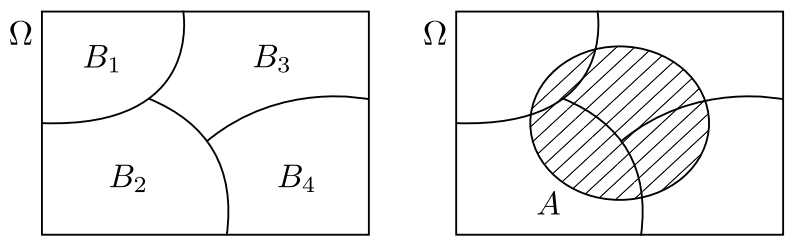
\includegraphics[width=\linewidth,keepaspectratio]{pictures/satz_der_totalen_wahrscheinlichkeit.png} 
\end{figure}

\DEF{Multiplikationsregel}{Seien $A_1,...,A_n\in\mathcal{F}$. Falls $\P[\bigcap_{i=1}^nA_i]>0$. Dann $\P[\bigcap_{i=1}^nA_i]=\P[A_1]\cdot\P[A_2|A_1]\cdot\P[A_3|A_1\cap A_2]\cdot ... \cdot\P[A_n|A_1\cap ...\cap A_{n-1}]$.}

\DEF{Satz von Bayes}{Sei $B_1, ...,B_N$ mit $\P[B_n]>0$ $\forall$ $n\in\{1,...,N\}$ eine Partition von $\Omega$. Dann $\forall$ $A\in\mathcal{F}$ mit $\P[A]>0$ gilt $\P[B_n|A]=\frac{\P[A|B_n]\P[B_n]}{\sum_{k=1}^N\P[A|B_k]\P[B_k]}$.}

\DEF{Satz von Bayes (Spezialfall $n=2$)}{$\P[B|A]=\frac{\P[A|B]\P[B]}{\P[A|B]\P[B] + \P[A|B^\complement]\P[B^\complement]}=\frac{\P[A\cap B]}{\P[A]}$.}




\mysubsection{Unabhängigkeit}
\DEF{Unabhängigkeit von 2 Ereignissen}{$A,B\in\mathcal{F}$ sind (stochastisch) unabhängig $\Leftrightarrow \P[A\cap B]=\P[A]\P[B] \Leftrightarrow \P[A|B]=\P[A] \Leftrightarrow \P[B|A]=\P[B]$.
\begin{itemize}
    \item $\P[A]\in\{0,1\} \Rightarrow \P[A\cap X]=\P[A]\P[X]$ $\forall$ $X\subseteq\mathcal{F} \Leftrightarrow A$ ist unabhängig von jedem Ereignis.
    \item $A$ ist unabhängig von sich selbst $\Leftrightarrow \P[A\cap A]=\P[A]^2 \Rightarrow \P[A]\in\{0,1\}$.
    \item $\P[A\cap B]=\P[A]\P[B] \Leftrightarrow \P[A\cap B^\complement]=\P[A]\P[B^\complement]$.
\end{itemize}}

\DEF{Unabhängigkeit von n Ereignissen}{Sei $I$ eine beliebige Indexmenge. Eine Familie von Ereignissen $(A_i)_{i\in I}$ ist (stochastisch) unabhängig $\Leftrightarrow $ $\forall$ $J\subset I$ gilt $\P[\bigcap_{j\in J}A_j]=\prod_{j\in J}\P[A_j]$.}

\DEF{Paarweise Unabhängigkeit}{Produktformel gilt nur für alle Paare von Ereignissen. Unabhängigkeit $\Rightarrow$ paarweise Unabhängigkeit $\not\Rightarrow$ Unabhängigkeit.}




\mysubsection{Zufallsvariablen}
\DEF{Zufallsvariable}{Eine (reellwertige) Zufallsvariable (ZV) ist eine Abbildung $X:\Omega\rightarrow\R$ $(\omega\mapsto X(\omega))$ s.d. $\forall$ $x\in\R$ gilt $\{\omega\in\Omega|X(\omega)\leq x\}\in\mathcal{F} \Leftrightarrow \{\omega\in\Omega|X(\omega)\in (-\infty,x]\}\in\mathcal{F} \Leftrightarrow \{\omega\in\Omega|X(\omega)\in B\}\in\mathcal{F}$ wobei $B=(-\infty,x]\in\mathcal{B}(\R) \Leftrightarrow X$ ist eine messbare Funktion.}

\DEF{Diskrete Zufallsvariable}{Eine ZV $X:\Omega\rightarrow\R$ heisst diskret, falls eine endliche oder abzählbare Menge $W\subset\R$ existiert, s.d. $\P[X\in W]=1$, wenn also die Werte von $X$ fast sicher in $W$ liegen.

Wenn $\Omega$ endlich oder abzählbar $\Rightarrow$ jede ZV $X:\Omega\rightarrow\R$ diskret.}

\DEF{Urbild}{Sei $X$ eine ZV. Sei $B\in\mathcal{B}(\R)$. Dann $X^{-1}(B):=\{\omega\in\Omega|X(\omega)\in B\}$ wobei für Messbarkeit $X^{-1}(B)\in\mathcal{F}$ $\forall B\in\mathcal{B}(\R)$ gelten muss.}

\DEF{Indikatorfunktion auf $A\in\mathcal{F}$}{
$1_A(\omega)=\begin{cases}
0 & \text{if } \omega\not\in A,\\
1 & \text{if } \omega\in A.
\end{cases}$

$\{\omega\in\Omega|1_A(\omega)\leq x\}=\begin{cases}
\emptyset & \text{if } x<0,\\
A^\complement & \text{if } 0\leq x< 1,\\
\Omega & \text{if } x\geq 1.
\end{cases}$
}

\DEF{Komposition}{Sei $X:\Omega\rightarrow\R$ eine ZV und $\phi:\R\rightarrow\R$ eine Funktion. Dann ist die Komposition $\phi(X):=\phi\circ X:\Omega\rightarrow\R$ ebenfalls eine ZV.
\begin{align*}
    \Omega \stackrel{X}{\rightarrow} \R& \stackrel{\phi}{\rightarrow}  \R\\
    \omega \mapsto X(\omega)& \mapsto  \phi(X(\omega))
\end{align*}
Für $n$ ZV $X_1,...,X_n$ und eine Abbildung $\phi:\R_n\rightarrow\R$ schreiben wir $\phi(X_1,...,X_n):=\phi\circ(X_1,...,X_n):\Omega\rightarrow\R$. Wobei $\phi$ eine Funktion mit mehreren Parametern ist.}

\DEF{Notation}{
\begin{align*}
    \{X\leq x\}&:=\{\omega\in\Omega|X(\omega)\leq x\},\\
    \{x<X\leq y\}&:=\{\omega\in\Omega|X(\omega)\in (x,y], x<y\},\\
    \{X\in\N\}&:=\{\omega\in\Omega|X(\omega)\in\N\},\\
    \hdots\\
    \P[X\leq x]&:=\P[\{X\leq x\}]=\P[\{\omega\in\Omega|X(\omega)\leq x\}],\\
    \hdots
\end{align*}}

\DEF{Unabhängigkeit}{Die ZV $X_1,...,X_n$ heissen unabhängig, wenn $\forall x_1,...,x_n\in\R$ gilt $\P[X_1\leq x_1,...,X_n\leq x_n]=\P[X_1\leq x_1]\cdot ... \cdot\P[X_n\leq x_n] \Leftrightarrow$ $\forall I_1\in\R,...,I_n\in\R$ die Ereignisse $\{X_1\in I_1\},...,\{X_n\in I_n\}$ unabhängig sind.}

\DEF{Gruppierung}{Seien $X_1,...,X_n$ unabhängige ZV. Seien $1\leq i_1 < i_2 < ... < i_k \leq n$ Indexe und $\phi_1,...\phi_k$ Abbildungen. Dann sind $Y_1:=\phi_1(X1,...,X_{i_1}),Y_2:=\phi_2(X_1,...,X_{i_2}),...,Y_k:=\phi_k(X_1,...,X_{i_k})$ unabhängig.}




\mysubsection{Verteilungsfunktion}
\DEF{Verteilungsfunktion (cumulative distribution function, cdf)}{Sei $X$ eine ZV auf $(\Omega,\mathcal{F},\P)$. Dann ist die cdf die Funktion $F_X:\R\rightarrow[0,1]$, definiert durch $x\mapsto F_X(x):=\P[X\leq x]$ und erfüllt folgende Eigenschaften:
\begin{enumerate}
    \item $F_X$ ist monoton wachsend.
    \item $F_X$ ist rechtsstetig, d.h. $\forall x\in\R$ gilt $F_X(x)=lim_{h\rightarrow 0}F_X(x+h)$.
    \item $lim_{x\rightarrow -\infty}F_X(x)=0$ und $lim_{x\rightarrow\infty}F_X(x)=1$.
\end{enumerate}}

\SA{}{Sei $X$ eine reellwertige ZV und seien $a,b\in\R$ mit $a<b$. Dann $\P[a<X\leq b]=F_X(b)-F_X(a)$.}

\DEF{Gemeinsame Verteilungsfunktion (joint cumulative distribution function, jcdf)}{Seien $X_1,...,X_n$ ZV. Dann ist die jcdf eine Abbildung $F:\R^n\rightarrow[0,1]$ definiert durch $(x_1,...,x_n)\mapsto F(x_1,...x_n)=\P[X_1\leq x_1,...,X_n\leq x_n]$.}

\DEF{Unabhängig und identisch verteilt (idependent and identically distributed, i.i.d.)}{Eine Folge von ZV $X_1,X_2,...$ heisst i.i.d. falls sie unabhängig ist und die ZV dieselbe cdf haben. d.h. $F_{X_k}=F_{X_l}$ $\forall$ $k,l\in\N$.}

\DEF{Unstetigkeit der Verteilungsfunktion}{Für $X\sim Ber(p)$ mit $p < 1$ gilt $\forall h>0$ $F_X(-h)=0$. Aber $F_X(0)=1-p\not = 0 \Leftrightarrow F$ nicht linksstetig in $0$. Also $lim_{h\rightarrow 0}F_U(-h)=0\not =F_X(0)$.}

\DEF{Linksseitiger Grenzwert im Punkt x}{$F(x-):=lim_{h\rightarrow 0}F(x-h)$.}

\DEF{Wahrscheinlichkeit eines Punktes}{Sei $X:\Omega\rightarrow\R$ eine ZV mit cdf $F$. Dann $\forall x\in\R$ gilt $\P[X=x]=F(x)-F(x-)=F(x)-lim_{h\rightarrow 0}F(x-h)$.}




\mysubsection{Konstruktion gleichverteilter ZV}
\DEF{Existenzsatz von Kolmogorov}{Es existiert ein $(\Omega,\mathcal{F},\P)$ und eine unendliche Folge von i.i.d. Bernoulli Zufallsvariablen $X_1,X_2,...$ auf $(\Omega,\mathcal{F},\P)$ mit Parameter $\frac{1}{2}$.}

\DEF{Gleichverteilt}{Sei $U$ eine ZV. $U$ ist gleichverteilt auf $[0,1]$ $\Leftrightarrow U\sim\mathcal{U}([0,1]) \Leftrightarrow F_U(x) = \begin{cases}
    0 & \text{if } x<0, \\
    x & \text{if } 0\leq x \leq 1, \\
    1 & \text{if } x > 1.
\end{cases}$}

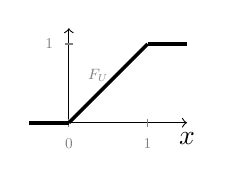
\begin{tikzpicture}
    \draw[->] (-0.5, 0) -- (1.5, 0) node[below] {$x$};
    \draw[->] (0, 0) -- (0, 1.2);
    \foreach \x in {0, 1} {
        \draw [gray] (\x, 0.05) -- ++(0, -.1) ++(0, -.15) node [below, outer sep=0pt, inner sep=0pt, scale=0.6] {\small\(\x\)};}
    \foreach \y in {1} {
        \draw [gray] (0.05, \y) -- ++(-.1, 0) ++(-.15, 0) node [left, outer sep=0pt, inner sep=0pt, scale=0.6] {\small\(\y\)};}
    \draw [gray] (0.5, 0.6) node [left, outer sep=0pt, inner sep=0pt, scale=0.6] {\small\(F_U\)};
    \draw[draw=black,line width=1.3pt] (-0.5,0) -- (0,0);
    \draw[draw=black,line width=1.3pt] (0,0) -- (1,1);
    \draw[draw=black,line width=1.3pt] (1,1) -- (1.5,1);
\end{tikzpicture}

\SA{}{Sei $X_1,X_2,...$ eine Folge unabhängiger Bernoulli-ZV mit Parameter $\frac{1}{2}$. Also $\forall \omega\in\Omega$ gilt $X_1(\omega),X_2(\omega),...\in\{0,1\}$. Somit konvergiert die Reihe $X(\omega):=\sum_{n=1}^{\infty}2^{-n}X_n(\omega)$ absolut. Weiter ist $X:\Omega\rightarrow[0,1]$ eine gleichverteilte ZV auf $[0,1]$.}

\DEF{Binärdarstellung}{Jedes $x\in[0,1)$ kann eindeutig in der Form $x=\sum_{n=1}^{\infty}2^{-n}x_n=\frac{1}{2}x_1+\frac{1}{4}x_2+\frac{1}{8}x_3+...$ dargestellt werden, wobei $x_n\in\{0,1\} \forall n\in\N$ und $\forall N\in\N \exists k>N$ s.d. $x_k=0$ (also die Folge "endet" nicht in unendlich vielen 1-en). Die Folge $\{x_n\}_{n\in\N}$ heisst Binärdarstellung von $x$ und wir schreiben $x=(.x_1x_2x_3...)_2$.}




\mysubsection{Konstruktion beliebig verteilter ZV}
\DEF{Verallgemeinerte Inverse}{Sei $F:\R\rightarrow[0,1]$ eine cdf. Dann ist die Abbildung $F^{-1}:(0,1)\rightarrow\R$ definiert durch $F^{-1}(\alpha)=inf\{x\in\R|F(x)\geq\alpha\}$ die verallgemeinerte inverse cdf von $F$.

Da $F$ rechtsstetig gilt $\forall x\in\R$ und $\alpha\in(0,1)$, dass $F^{-1}(\alpha)\leq x\Leftrightarrow \alpha\leq F(x)$.}

\DEF{Inversionsmethode}{Sei $F:\R\rightarrow [0,1]$ eine cdf. Sei $U\sim\mathcal{U}([0,1])$. Dann hat die ZV $X:=F^{-1}(U)$ die cdf $F$.}

\SA{}{Sei $F_1,F_2,...$ eine Folge von cdf. Dann $\exists (\Omega,\mathcal{F},\P)$ und eine Folge von ZV $X_1,X_2,...$ auf $(\Omega,\mathcal{F},\P)$, s.d. $\forall k\in\N$ gilt $X_k$ hat cdf $F_k$ und $X_1,X_2,...$ sind unabhängig.}



\mysubsection{Gewichtsfunktion}
\DEF{Gewichtsfunktion (diskrete dichte, probability mass function, pmf)}{Sei $X$ mit Wertebereich $W(X)=\{x_1,x_2,...\}$ und den dazugehörigen Wahrscheinlichkeiten $\{p1,p2,...\}$ eine diskrete ZV. Dann ist die pmf definiert als $p_X:W(X)\rightarrow[0,1]$ mit $p_X(x_k):=\P[X=x_k]=p_k$ und hat folgende Eigenschaften:
\begin{itemize}
    \item $\forall x_k\in W(X)$ gilt $p_X(x_k)\in[0,1]$.
    \item $\sum_{x_k\in W(X)}p_X(x_k)=\P[X\in W(X)]=1$.
\end{itemize}

Die Zahlenfolge $\{p_X(x_k)\}_{x_k\in W(X)}$ wird auch Verteilung von $X$ genannt.}

\SA{}{Sei $X$ eine diskrete ZV mit Werten in $W$ und pmf $p_X$. Dann ist die cdf von $X$ gegeben durch $F_X(x)=\P[X\leq x]=\sum_{y\in W,y\leq x}p_X(y)$. Weiter gilt für jede messbare Teilmenge $B\subseteq W$, dass $\P[X\in B]=\sum_{x\in B}p_X(x)$.}

\DEF{Gemeinsame Gewichtsfunktion}{Seien $X,Y$ diskrete ZV mit Wertebereichen $W_X$ und $W_Y$. Seien $x\in W_X,y\in W_Y$. Dann ist ihre gemeinsame pmf definiert als $p_{X,Y}: W_X\times W_Y\rightarrow[0,1]$ mit $p_{X,Y}(x,y):=\P[X=x,Y=y]$.}

\DEF{Randgewicht}{Seien $X,Y$ diskrete ZV mit Wertebereichen $W_X$ und $W_Y$. Sei $x\in W_X$. Dann ist das Randgewicht von $X$ definiert als $p_X(x)=\sum_{y\in W_Y}f_{X,Y}(x,y)$.}


\mysubsection{Diskrete Verteilungen}
\DEF{Bernoulli}{Sei $p\in[0,1]$. ZV $X$ ist Bernoulli ZV mit parameter $p \Leftrightarrow X\sim Ber(p) \Leftrightarrow$ $\forall\omega\in\Omega: X(\omega)\in\{0,1\}=W_X\ \land$\\ $\forall k\in W_X: p_X(k)=\P[X=k]=\begin{cases}
    p & \text{if $k=1$,}\\
    1-p & \text{if $k=0$.}
\end{cases}$ 

\begin{enumerate}
    \item $\E[X]=p$.
    \item $\V[X]=p(1-p)$.
\end{enumerate}}

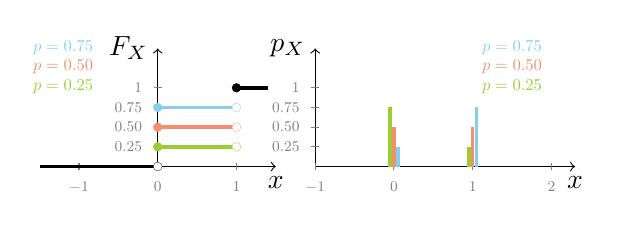
\begin{tikzpicture}
\begin{scope}
    % Axis
    \draw[->] (-1.5, 0) -- (1.5, 0) node[below]{$x$};
    \draw[->] (0, 0) -- (0, 1.5) node[left]{$F_X$};

    % Axis labels
    \foreach \x in {-1, ..., 1} {
        \draw [gray] (\x, 0.05) -- ++(0, -.1) ++(0, -.15) node [below, outer sep=0pt, inner sep=0pt, scale=0.6] {\small\(\x\)};}
    \foreach \y in {0.25, 0.50, 0.75, 1} {
        \draw [gray] (0.05, \y) -- ++(-.1, 0) ++(-.15, 0) node [left, outer sep=0pt, inner sep=0pt, scale=0.6] {\small\(\y\)};}

    % Definitions
    \def\pOne {0.25}
    \def\pTwo {0.50}
    \def\pThree {0.75}

    \def\firstColor {YellowGreen};
    \def\secondColor {Melon};
    \def\thirdColor {SkyBlue};
    
    % Legend
    \node [above, text=\firstColor,scale=0.6] at (-1.2,\pOne + 0.6) {$p = \pOne$};
    \node [above, text=\secondColor,scale=0.6] at (-1.2,\pTwo + 0.6) {$p = \pTwo$};
    \node [above, text=\thirdColor,scale=0.6] at (-1.2,\pThree + 0.6) {$p = \pThree$};
    
    % Function
    \draw[draw=black,line width=1.3pt] (-1.5,0) -- (0,0);
    \filldraw[draw=black,line width=0.1pt,fill=white] (0,0) circle[radius=1.6pt];

    \draw[draw=\firstColor,line width=1.3pt] (0,\pOne) -- (1,\pOne);
    \filldraw[draw=\firstColor,line width=0.1pt,fill=\firstColor] (0,\pOne) circle[radius=1.6pt];
    \filldraw[draw=\firstColor,line width=0.1pt,fill=white] (1,\pOne) circle[radius=1.6pt];

    \draw[draw=\secondColor,line width=1.3pt] (0,\pTwo) -- (1,\pTwo);
    \filldraw[draw=\secondColor,line width=0.1pt,fill=\secondColor] (0,\pTwo) circle[radius=1.6pt];
    \filldraw[draw=\secondColor,line width=0.1pt,fill=white] (1,\pTwo) circle[radius=1.6pt];

    \draw[draw=\thirdColor,line width=1.3pt] (0,\pThree) -- (1,\pThree);
    \filldraw[draw=\thirdColor,line width=0.1pt,fill=\thirdColor] (0,\pThree) circle[radius=1.6pt];
    \filldraw[draw=\thirdColor,line width=0.1pt,fill=white] (1,\pThree) circle[radius=1.6pt];
    
    \draw[draw=black,line width=1.3pt] (1,1) -- (1.4,1);
    \filldraw[draw=black,line width=0.1pt,fill=black] (1,1) circle[radius=1.6pt];
\end{scope}
\begin{scope}[xshift=3cm]
    % Axis
    \draw[->] (-1, 0) -- (2.3, 0) node[below]{$x$};
    \draw[->] (-1, 0) -- (-1, 1.5) node[left]{$p_X$};

    % Axis labels
    \foreach \x in {-1, ..., 2} {
        \draw [gray] (\x, 0.05) -- ++(0, -.1) ++(0, -.15) node [below, outer sep=0pt, inner sep=0pt, scale=0.6] {\small\(\x\)};}
    \foreach \y in {0.25, 0.50, 0.75, 1} {
        \draw [gray] (-0.95, \y) -- ++(-.1, 0) ++(-.15, 0) node [left, outer sep=0pt, inner sep=0pt, scale=0.6] {\small\(\y\)};}

    % Definitions
    \def\pOne {0.25}
    \def\pTwo {0.50}
    \def\pThree {0.75}

    \def\firstColor {YellowGreen};
    \def\secondColor {Melon};
    \def\thirdColor {SkyBlue};
    
    % Legend
    \node [above, text=\firstColor,scale=0.6] at (1.5,\pOne + 0.6) {$p = \pOne$};
    \node [above, text=\secondColor,scale=0.6] at (1.5,\pTwo + 0.6) {$p = \pTwo$};
    \node [above, text=\thirdColor,scale=0.6] at (1.5,\pThree + 0.6) {$p = \pThree$};
    
    % Function
    \draw[draw=\firstColor,line width=1.3pt] (-0.05,0) -- (-0.05,1-\pOne);
    \draw[draw=\secondColor,line width=1.3pt] (0,0) -- (0,1-\pTwo);
    \draw[draw=\thirdColor,line width=1.3pt] (0.05,0) -- (0.05,1-\pThree);    

    \draw[draw=\firstColor,line width=1.3pt] (0.95,0) -- (0.95,\pOne);    
    \draw[draw=\secondColor,line width=1.3pt] (1,0) -- (1,\pTwo);
    \draw[draw=\thirdColor,line width=1.3pt] (1.05,0) -- (1.05,\pThree);
\end{scope}
\end{tikzpicture}
\DEF{Binomialverteilung}{Modelliert die Anzahl Erfolge bei wiederholten Bernoulli-Experimenten. Sei $p\in[0,1]$ und $n\in\N$. ZV $X$ ist binomialverteilt mit Parametern $n$ und $p$ $\Leftrightarrow$ $X\sim Bin(n,p) \Leftrightarrow$ $\forall\omega\in\Omega: X(\omega)\in\{0,...,n\}=W_X\ \land\ \forall k\in W_X:p_X(k)=\P[X=k]={n\choose k} p^k(1-p)^{n-k}$.

\begin{enumerate}
    \item $\E[X]=np$.
    \item $\V[X]=np(1-p)$.
\end{enumerate}}

\SA{}{Sei $p\in[0,1]$ und $n\in\N$. Seien $X_1,...,X_n\sim Ber(p)$ alle unabhängig. Dann gilt $S_n:=X_1+...+X_n\sim Bin(n,p)$.}

\DEF{Geometrische Verteilung}{Sei $p\in(0,1]$. ZV $X$ ist geometrisch verteilt mit Parameter $p \Leftrightarrow X\sim Geom(p) \Leftrightarrow \forall\omega\in\Omega: X(\omega)\in\N=W_X\ \land\ \forall k\in W_X:p_X(k)=\P[X=k]=p(1-p)^{k-1}$. Für den Fall $p=1$ und $k=1$ erhalten wir einen Term $0^0$. Wir verwenden die Konvention $0^0=1$ und damit gilt $\P[X=1]=p$. 

\begin{enumerate}
    \item $F_X(x)=1-(1-p)^{x}$.
    \item $\E[X]=\frac{1}{p}$.
    \item $\V[X]=\frac{1-p}{p^2}$.
    \item Intuition: Modelliert die Wartezeit bis zum ersten Erfolg in einer unendlichen Folge von Bernoulli-Experimenten.
    \item Gedächtnislosigkeit: $\forall n \geq 0$ und $\forall k\geq 1$ gilt $\P[T\geq n+k|T>n]=\P[T\geq k]$.
\end{enumerate}}

\SA{}{Sei $X_1,X_2,...$ eine unendliche Folge von unabhängigen Bernoulli-Zufallsvariablen mit Parameter $p$. Dann ist $T:=inf\{n\geq 1|X_n=1\} \Rightarrow T\sim Geom(p)$.}

\DEF{Negativbinomiale Verteilung}{Verallgemeinerung der geom. Verteilung. Modelliert die Wartezeit bis zum $r$-ten Erfolg in einer unendlichen Folge von Ber.-Experimenten. ZV $X$ ist negativbinomial verteilt mit $r\in\N$ und $p\in[0,1] \Leftrightarrow X\sim NBin(r,p) \Leftrightarrow$ $\forall\omega\in\Omega: X(\omega)\in\{r,r+1,r+2,...\}=W_X\ \land\ \forall k\in W_X:p_X(k)=\P[X=k]={{k-1}\choose{r-1}}p^r(1-p)^{k-r}$. 

\begin{enumerate}
    \item $\E[X]=$.
    \item $\V[X]=$.
\end{enumerate}}

\SA{}{Sei $X_1,X_2,...$ eine unendliche Folge von unabhängigen Bernoulli-Zufallsvariablen mit Parameter $p$. Dann ist $T_r:=inf\{n\geq 1|\sum_{l=1}^nX_l=r\} \Rightarrow T_r\sim NBin(r,p)$.}

\SA{}{Seien $X_1,...,X_r\sim Geom(p)$ und unabhängige ZV. Dann ist ihre Summe $X=X_1+...+X_r\sim NBin(r,p)$.}

\DEF{Hypergeometrische Verteilung}{Seien in einer Urne $n$ Gegenstände, davon $r$ vom Typ 1 und $n-r$ vom Typ 2. Man ziehe $m$ Gegenstände ohne Zurücklegen. Dann ist ZV $X\sim H(n,r,m)$ die \# gezogener Gegenstände $k$ vom Typ 1. ZV $X$ ist hypergeometrisch verteilt mit Parametern $n\in\N$, $m,r\in\{1,...,n\} \Leftrightarrow X\sim H(n,r,m) \Leftrightarrow$ $\forall k\in\{0,1,...,min(m,r)\}$ gilt $\P[X=k]=\frac{{r\choose k}{n-r\choose m-k}}{{n\choose m}}$.

\begin{enumerate}
    \item $\E[X]=$.
    \item $\V[X]=$.
\end{enumerate}}

\DEF{Poisson-Verteilung}{Grenzwert der Binomial-Verteilung. Sei $\lambda\in\R,\lambda>0$. ZV $X$ ist Poisson-verteilt mit Parameter $\lambda \Leftrightarrow X\sim Poisson(\lambda) \Leftrightarrow \forall\omega\in\Omega:X(\omega)\in\N_0=W_X\ \land\ \forall k\in\N_0:p_X(k)=\P[X=k]=\frac{\lambda^k}{k!}e^{-\lambda}=\frac{e^{-\lambda}\lambda^k}{k!}$.

\begin{enumerate}
    \item $\E[X]=\V[X]=\lambda$.
\end{enumerate}}

\SA{}{Sei $\lambda > 0$. $\forall n\geq 1$ betrachten wir $n$ ZV $X_n\sim Bin(n,\lambda)$. Sei $N\sim Poisson(\lambda)$. Dann gilt $\forall k\in\N$, $lim_{n\rightarrow\infty}\P[X_n=k]=\P[N=k]$.}

\SA{}{Seien $X,Y$ reellwertige unabhängige ZV. Seien $\lambda,\mu>0$. Wenn $X\sim\mathcal{P}(\lambda), Y\sim\mathcal{P}(\mu)$ $\Rightarrow$ $X+Y\sim\mathcal{P}(\lambda+\mu)$.}



\mysubsection{Stetige Verteilungen}
\DEF{Stetig verteilte Zufallsvariable und Dichtefunktion (probability density function, pdf)}{ZV $X$ heisst stetig $\Leftrightarrow \exists f_X:\R\rightarrow\R_+:F_X(x)=\int_{-\infty}^xf_X(t)dt$. Wir nennen $f_X$ die pdf von $X$. Intuition: $f_X(t)dt$ ist die Wahrscheinlichkeit, dass $X\in[t,t+dt]$.}

\DEF{Stückweise stetig differenzierbare Funktionen}{Funktion $f$ ist stückweise stetig differenzierbar $\Leftrightarrow\ \exists$ eine Partition $-\infty = x_0 < x_1 < ... < x_{n-1} < x_n = \infty$ s.d. $f$ auf jedem Intervall $(x_i,x_{i+1})$ stetig differenzierbar ist.}

\SA{3.39.}{Sei $X$ eine ZV. Sei $F_X$ stetig und stückweise stetig differenzierbar auf einer Partition $-\infty=x_0<x_1<...<x_{n-1}<x_n=\infty \Rightarrow X$ ist eine stetige ZV und $f_X=\begin{cases}
    F_X'(x) & \text{if $\exists k\in\{0,...,n-1\}:x\in(x_k,x_{k+1}),$}\\
    a_k & \text{if $x\in\{x_1,...,x_{n-1}\},$}
\end{cases}$ wobei $a_k$ beliebig gewählt werden dürfen. Es gilt also $f_X(x)=F_X'(x)$ in allen Stetigkeitspunkten $x$ von $f_X$.}

\NOTE{$f_X$ vs. $p_X$}{Die pdf $f_X$ ist (fast exakt) das stetige Analogon zur pmf $p_X$ einer diskreten ZV.

\begin{enumerate}
    \item Für messbare Mengen $B\subset\R$ gilt $\P[X\in B]=\int_Bf_X(x)dx$ analog zu $\P[X\in B]=\sum_{x\in B}p_X(x)$.
    \item Da allerdings $\P[X=x]=0\ \forall x\in\R$, hat in diesem Sinn $X$ keine pmf wie diskrete ZV.
    \item Ist $f_X$ allerdings stetig an der Stelle $x$, so haben wir $f_X(x)=lim_{\varepsilon\rightarrow 0}\frac{1}{\varepsilon}\int_x^{x+\varepsilon}f_X(t)dt=lim_{\varepsilon\rightarrow0}\frac{\P[x<X\leq x+\varepsilon]}{\varepsilon}$ und somit $\P[X\in(x,x+\varepsilon)]\approx\varepsilon f_X(x)$ für kleine $\varepsilon$. Dies wird oft auch als $\P[X\in(x,x+dx]]=f_X(x)dx$ geschriben.
    \item Nach Satz 3.39 gilt für stetige Dichten, dass Verteilungsfunktion und Dichte auseinander durch Integrieren bzw. Differenzieren entstehen.
    \item Merkregel: Vom diskreten zum stetigen Fall kommt man, indem man die Kombination (Summe, Gewichtsfunktion bzw. pmf) systematisch durch (Integral, Dichtefunktion bzw. pdf) ersetzt.
\end{enumerate}}

\DEF{Gleichverteilung}{ZV $X$ ist gleichverteilt auf $[a,b] \Leftrightarrow X\sim\mathcal{U}([a,b]) \Leftrightarrow f_X(x)=\begin{cases}
    \frac{1}{b-a} & \text{$x\in[a,b],$}\\
    0 & \text{sonst.}
\end{cases}$

\begin{figure}[H]
 \centering
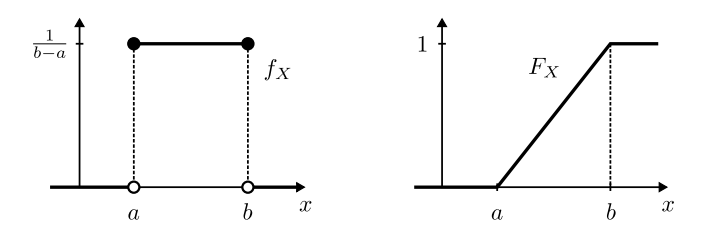
\includegraphics[width=\linewidth,keepaspectratio]{pictures/uniform_distribution.png} 
\end{figure}

\begin{enumerate}
    \item $\E[X]=\frac{a+b}{2}$.
    \item $\V[X]=\frac{(b-a)^2}{12}$.
    \item Intuition: Modelliert die zufällige Wahl eines Punktes in $[a,b]$.
\end{enumerate}}

\DEF{Exponentialverteilung}{ZV $X$ ist exponentialverteilt mit $\lambda > 0 \Leftrightarrow X\sim Exp(\lambda) \Leftrightarrow$ $\forall x\in\R:f_X(x)=\begin{cases}
    \lambda e^{-\lambda x} & \text{$x\geq 0,$}\\
    0 & \text{$x<0.$}
\end{cases}$

\begin{figure}[H]
 \centering
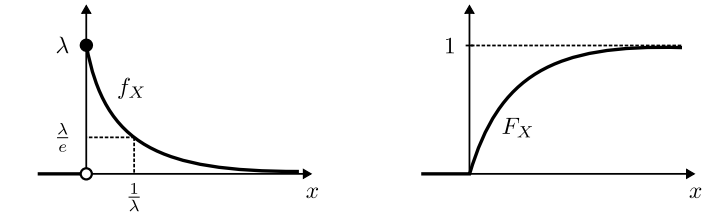
\includegraphics[width=\linewidth,keepaspectratio]{pictures/exponential_distribution.png} 
\end{figure}

\begin{enumerate}
    \item $F_X(x)=1-e^{-\lambda x}\Leftrightarrow F_X^{-1}(y)=\frac{-1}{\lambda}log(1-y)$.
    \item $\E[X]=\frac{1}{\lambda}$.
    \item $\V[X]=\frac{1}{\lambda^2}$.
    \item Intuition: Ist das stetige Analogon der geometrischen Verteilung. Modelliert die Wartezeit oder Lebensdauer für beliebige Werte $x\geq 0$.
    \item Besitzt auch die Eigenschaft der Gefächtnislosigkeit, also $\P[X>t+s|X>s]=\P[X>t]$.
\end{enumerate}}

\DEF{Cauchy-Verteilung}{ZV $X$ ist Cauchy-verteilt mit $x_0\in\R,\gamma > 0 \Leftrightarrow X\sim Cauchy(x_0,\gamma) \Leftrightarrow$ $f_X(x)=\frac{1}{\pi}\frac{\gamma}{\gamma^2+(x-x_0)^2}$.
\begin{figure}[H]
 \centering
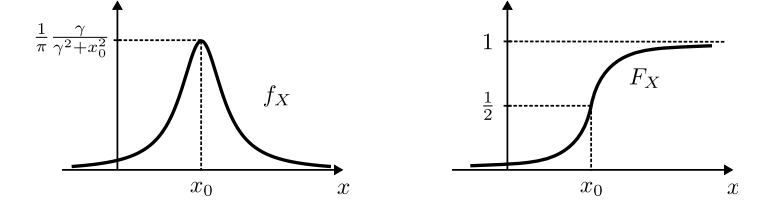
\includegraphics[width=\linewidth,keepaspectratio]{pictures/cauchy_distribution.png} 
\end{figure}

\begin{enumerate}
    \item $F_X(x)=\frac{1}{2}+\frac{1}{\pi}\arctan(x)\Leftrightarrow F_X^{-1}(y)=\tan((y-\frac{1}{2})\pi)$.
    \item $\E[X]$ undefiniert, $\E[X_+]=\E[X_-]=\infty$.
    \item Weiter gilt $F_X(x)=\frac{1}{2}+\frac{1}{\pi}arctan(\frac{x-x_0}{\gamma})$.
    \item $Y,Z$ unabhängige $\mathcal{N}(0,1)$-verteilte ZV $\Rightarrow \frac{Y}{Z}=X\sim Cauchy(0,1)$.
    \item Ist eine langschwänzige Verteilung (heavytailed distribution). $f_X(x)$ geht für $|x|\rightarrow\infty$ nur sehr langsam gegen 0 (quadratisch, im Vergelich zum exponentiellen Abfallen bei der Normalverteilung).
\end{enumerate}}

\DEF{Normalverteilung}{ZV $X$ ist normalverteilt mit $\mu\in\R,\sigma^2>0 \Leftrightarrow X\sim\mathcal{N}(\mu,\sigma^2) \Leftrightarrow$ $f_X(x)=\frac{1}{\sigma\sqrt{2\pi}}e^{-\frac{1}{2}(\frac{x-\mu}{\sigma})^2}$.
\begin{figure}[H]
 \centering
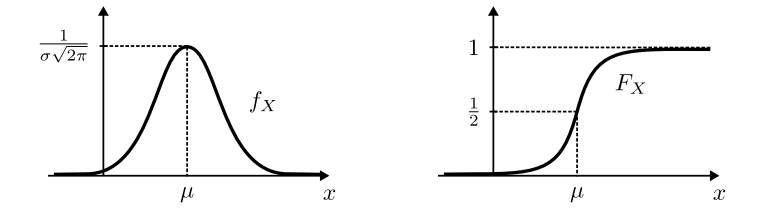
\includegraphics[width=\linewidth,keepaspectratio]{pictures/normal_distribution.png} 
\end{figure}

\begin{enumerate}
    \item $\E[X]=\mu$.
    \item $\V[X]=\sigma^2$.
    \item Wird auch als gausssche Glockenkurve, Gauss-Funktion, gausssche Normalverteilung, gausssche Verteilungskurve, Gauss-Kurve, und Gauss-Glocke bezeichnet.
    \item $f_X=\varphi$ und $F_X=\Phi$. Die zugehörigen Variablen nennen wir $Z$.
    \item Weder für $F_X$ noch für $\Phi$ gibt es einen geschlossenen Ausdruck, aber das Integral $\Phi(x)=\int_{-\infty}^x\varphi(t)dt=\frac{1}{\sqrt{2\pi}}\int_{-\infty}^xe^{-\frac{t^2}{2}}dt$ ist tabelliert.
    \item Uneigentliches Integral über Normalverteilung (L4.21): $\int_{-\infty}^{\infty}e^{\frac{-x^2}{2\sigma^2}}dx=\sqrt{2\pi\sigma^2}$.
\end{enumerate}}

\DEF{Standardnormalverteilung}{Wichtiger Spezialfall der Normalverteilung mit $\mu=0, \sigma^2=1$ also $\mathcal{N}(0,1)$. Für $X\sim\mathcal{N}(\mu,\sigma^2)$ gilt $\frac{X-\mu}{\sigma}\sim\mathcal{N}(0,1),$ also $F_X(x)=\P[X\leq x]=\P[\frac{X-\mu}{\sigma}\leq\frac{x-\mu}{\sigma}]=\Phi(\frac{x-\mu}{\sigma})$. Daraus folgt, dass für $\mu\in\R,\sigma^2>0,Z\sim\mathcal{N}(0,1)$ gilt $\mu+\sigma Z\sim\mathcal{N}(\mu,\sigma^2)$.

Es gilt $\E[X^{2k}]=(2k-1)!!$, wobei $(2k-1)!!$ die Doppelfakultät ist, also das Produkt aller ungeraden Zahlen.

Um jede beliebig normalverteilte ZV $X\sim\mathcal{N}(\mu,\sigma^2)$ zu simulieren, reicht es $Z\sim\mathcal{N}(0,1)$ zu simulieren und die erhaltetnen Werte mit $\sigma$ zu multiplizieren und mit $\mu$ zu addieren.}

\SA{3.50.}{Seien $X_1,...,X_n$ unabhängige ZV s.d. $X_1\sim\mathcal{N}(\mu_1,\sigma_1^2),...,X_n\sim\mathcal{N}(\mu_n,\sigma_n^2)$. Dann $Z:=\mu_0+\sum_{k=1}^na_kX_k\sim\mathcal{N}(\mu_0+\sum_{k=1}^na_k\mu_k,\sum_{k=1}^na_k^2\sigma_k^2)$.}

\SA{3.52.}{Für $X\sim\mathcal{N}(\mu,\sigma^2)$ liegt der "Grossteil" des Wahrscheinlichkeitsmasses im Intervall $[\mu-3\sigma,\mu+3\sigma]$. Es gilt $\P[|X-\mu|\geq 3\sigma]\leq 0.0027$.}
